
\section{Application to Observations}
\label{dga:sec:h3}

We now apply our likelihood function (Eq.~\ref{dga:eq:likelihood}) to two
disrupted dwarf galaxies in the Milky Way stellar halo.
The first is a relatively well-studied system: GSE~\citep{Belokurov2018,
Helmi2018, Haywood2018, Myeong2018, Mackereth2019}, believed to be responsible
for a major merger event early in the Milky Way's history~\citep{Gallart2019,
Bonaca2020, Chaplin2020, Montalban2021, Xiang2022} which
contributed~$\sim$$10^9~\msun$ of total stellar mass to the Galaxy
\citep{Deason2019, Fattahi2019, Mackereth2019, Vincenzo2019b, Kruijssen2020,
Han2022}, including eight globular clusters in the stellar
halo~\citep{Myeong2018, Massari2019, Kruijssen2019, Forbes2020}.
GSE is a good test case for this method both because it is the dominant
structure in the Milky Way's inner halo~\citep{Helmi2018} and because we can
compare to independent constraints thanks to the amount of attention it has
received in the literature.

\subfile{results.tablebody.tex}

The second is a less well-studied system: Wukong/LMS-1, a structure chemically
distinct from GSE which sits between it and the Helmi stream~\citep{Helmi1999}
in energy-angular momentum space~\citep{Naidu2020, Yuan2020} that
formed from an M$_\star \approx \scinote{1.3}{7}~\msun$ disrupted
galaxy~\citep{Naidu2022}.
Wukong/LMS-1 is an interesting system to investigate with our method
because it displays a ``classic'' enrichment history with an obvious ``knee''
in the evolutionary track near~$\feh \approx -2.8$ (see Fig.~\ref{dga:fig:wukong}
below).
It has been associated~\citep{Malhan2022} with the most metal-poor streams in
the halo~\citep[e.g.,][]{Roederer2019, Wan2020, Martin2022} and a high fraction
of carbon-enhanced metal-poor stars given its low stellar mass
\citep{Shank2022, Zepeda2023}, marking it as a disrupted dwarf with a
potentially remarkable chemical history.
We make use of data from the H3 survey (see discussion
in~\S~\ref{dga:sec:h3:survey} below) and discuss our GCE model fits to GSE and
Wukong/LMS-1 in~\S\S~\ref{dga:sec:h3:gse} and~\ref{dga:sec:h3:wukong}, comparing our
results for the two galaxies in~\S~\ref{dga:sec:h3:comparison}.

\subsection{The H3 Survey}
\label{dga:sec:h3:survey}

The H3 survey~\citep{Conroy2019} is collecting medium-resolution spectra
of~$\sim$300,000 stars in high-latitude fields ($\left|b\right| > 20^\circ$).
Spectra are collected from the Hectochelle instrument on the MMT
\citep{Szentgyorgyi2011}, which delivers~$R \approx$~32,000 spectra over the
wavelength range of~$5150 - 5300$~\AA.
Spectral lines in this wavelength range are dominated by iron-peak elements and
the MgI triplet (see Fig. 6 of~\citealt{Conroy2019}).
Throughout this section, the alpha element abundances we refer to are therefore
Mg abundances specifically, whereas in previous sections an alpha element
refers to any species where the only statistically significant enrichment
source is a metallicity-dependent yield from massive stars.
\par
The survey selection function is deliberately simple: the primary sample
consists of stars with~$r$ band magnitudes of~$15 < r < 18$
and~\gaia~\citep{GaiaCollaboration2016} parallaxes~$<$ 0.3 mas (this threshold
has evolved over the course of the survey as the~\gaia~astrometry has become
more precise).
Stellar parameters are estimated by the~\textsc{MINESweeper} program
\citep{Cargile2020}, which fits grids of isochrones, synthetic spectra and
photometry to the Hectochelle spectrum and broadband photometry from~\gaia,
Pan-STARRS~\citep{Chambers2016}, SDSS~\citep{York2000}, 2MASS
\citep{Skrutskie2006} and WISE~\citep{Wright2010} with the~\gaia~parallax
used as a prior.
The fitted parameters include radial velocity, spectrophotometric distance,
reddening,~\feh,~\afe~and age.
The default analysis includes a complicated prior on age and distance
(see~\citealt{Cargile2020} for details).
We have also re-fit high signal-to-noise data with a flat age prior for cases
where ages play an important role.
In this paper we use the catalog which uses this flat age prior.

\subsection{\gaia-Sausage Enceladus}
\label{dga:sec:h3:gse}

% fig 5
\begin{figure*}
\centering
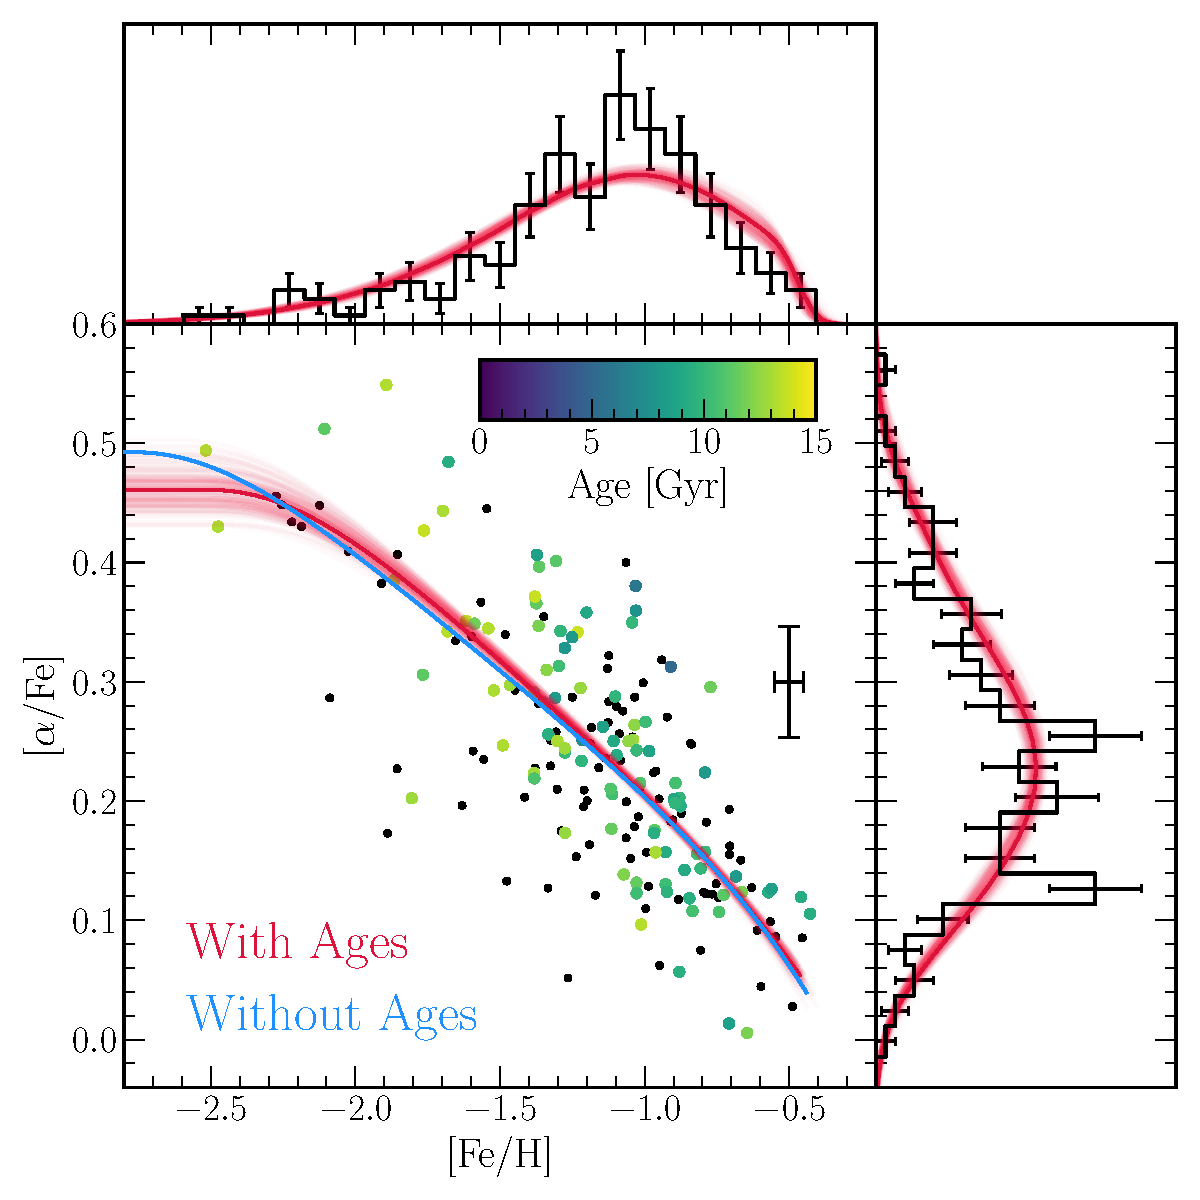
\includegraphics[scale = 0.65]{gsefit_afe_feh.pdf}
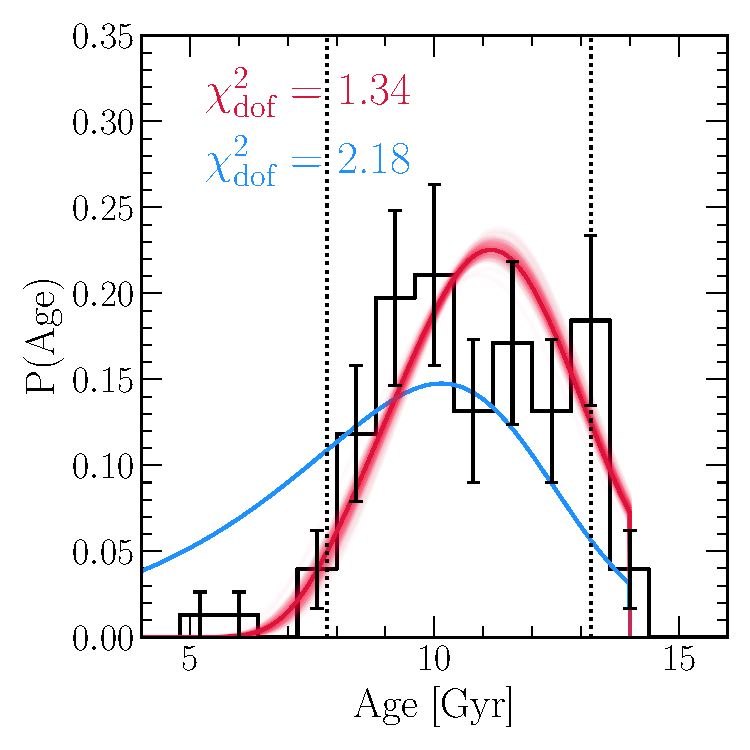
\includegraphics[scale = 0.54]{gsefit_agedist.pdf}
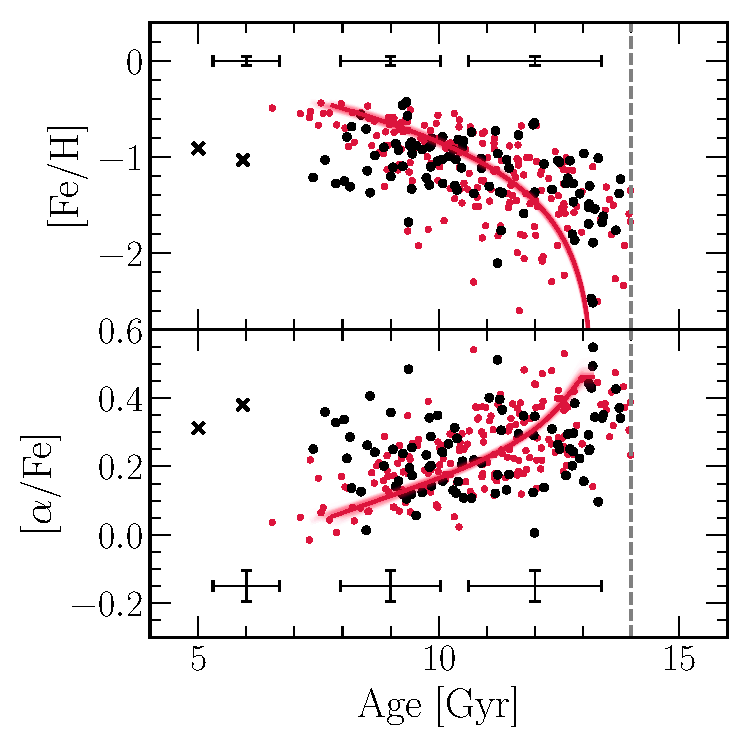
\includegraphics[scale = 0.53]{gsefit_amr.pdf}
\caption{
Our GSE sample.
Red lines in all panels denote the best-fit one-zone model, while the
blue lines in the top and bottom left panels denote the best-fit model obtained
when excluding age measurements from the fit.
Distributions in~\feh,~\afe~and age are convolved with the median uncertainty
of the sample (see discussion in~\S~\ref{dga:sec:h3:gse}).
We additionally subsample 200 sets of parameter choices from our Markov chain
and plot their predictions as highly transparent lines to offer a sense of the
fit uncertainty.
Error bars in each distribution indicate a~$\sqrt{N}$ uncertainty associated
with random sampling.
\textbf{Top}: Our sample in chemical space and the associated marginalized
distributions.
Stars with age measurements are colour coded accordingly and are otherwise
plotted in black.
The median~\feh~and~\afe~uncertainty in the sample is shown by the error bar
to the right of the data.
\textbf{Bottom left}: The age distribution of our GSE sample (black,
binned).
\textbf{Bottom right}: Age-\feh~(top) and age-\afe~(bottom) relations
The median~\feh,~\afe~and age uncertainties are shown by the error bars at the
top and bottom of each panel.
We plot the two stars that we exclude from our fit as black X's (likely
blue stragglers; see discussion in~\S~\ref{dga:sec:h3:gse}).
Red points denote~$N = 95$ stars (the same size as the stars with ages in our
GSE sample) drawn from out best-fit model and perturbed by the median age
uncertainty of the sample.
}
\label{dga:fig:gse}
\end{figure*}

% fig 6
\begin{figure*}
\centering
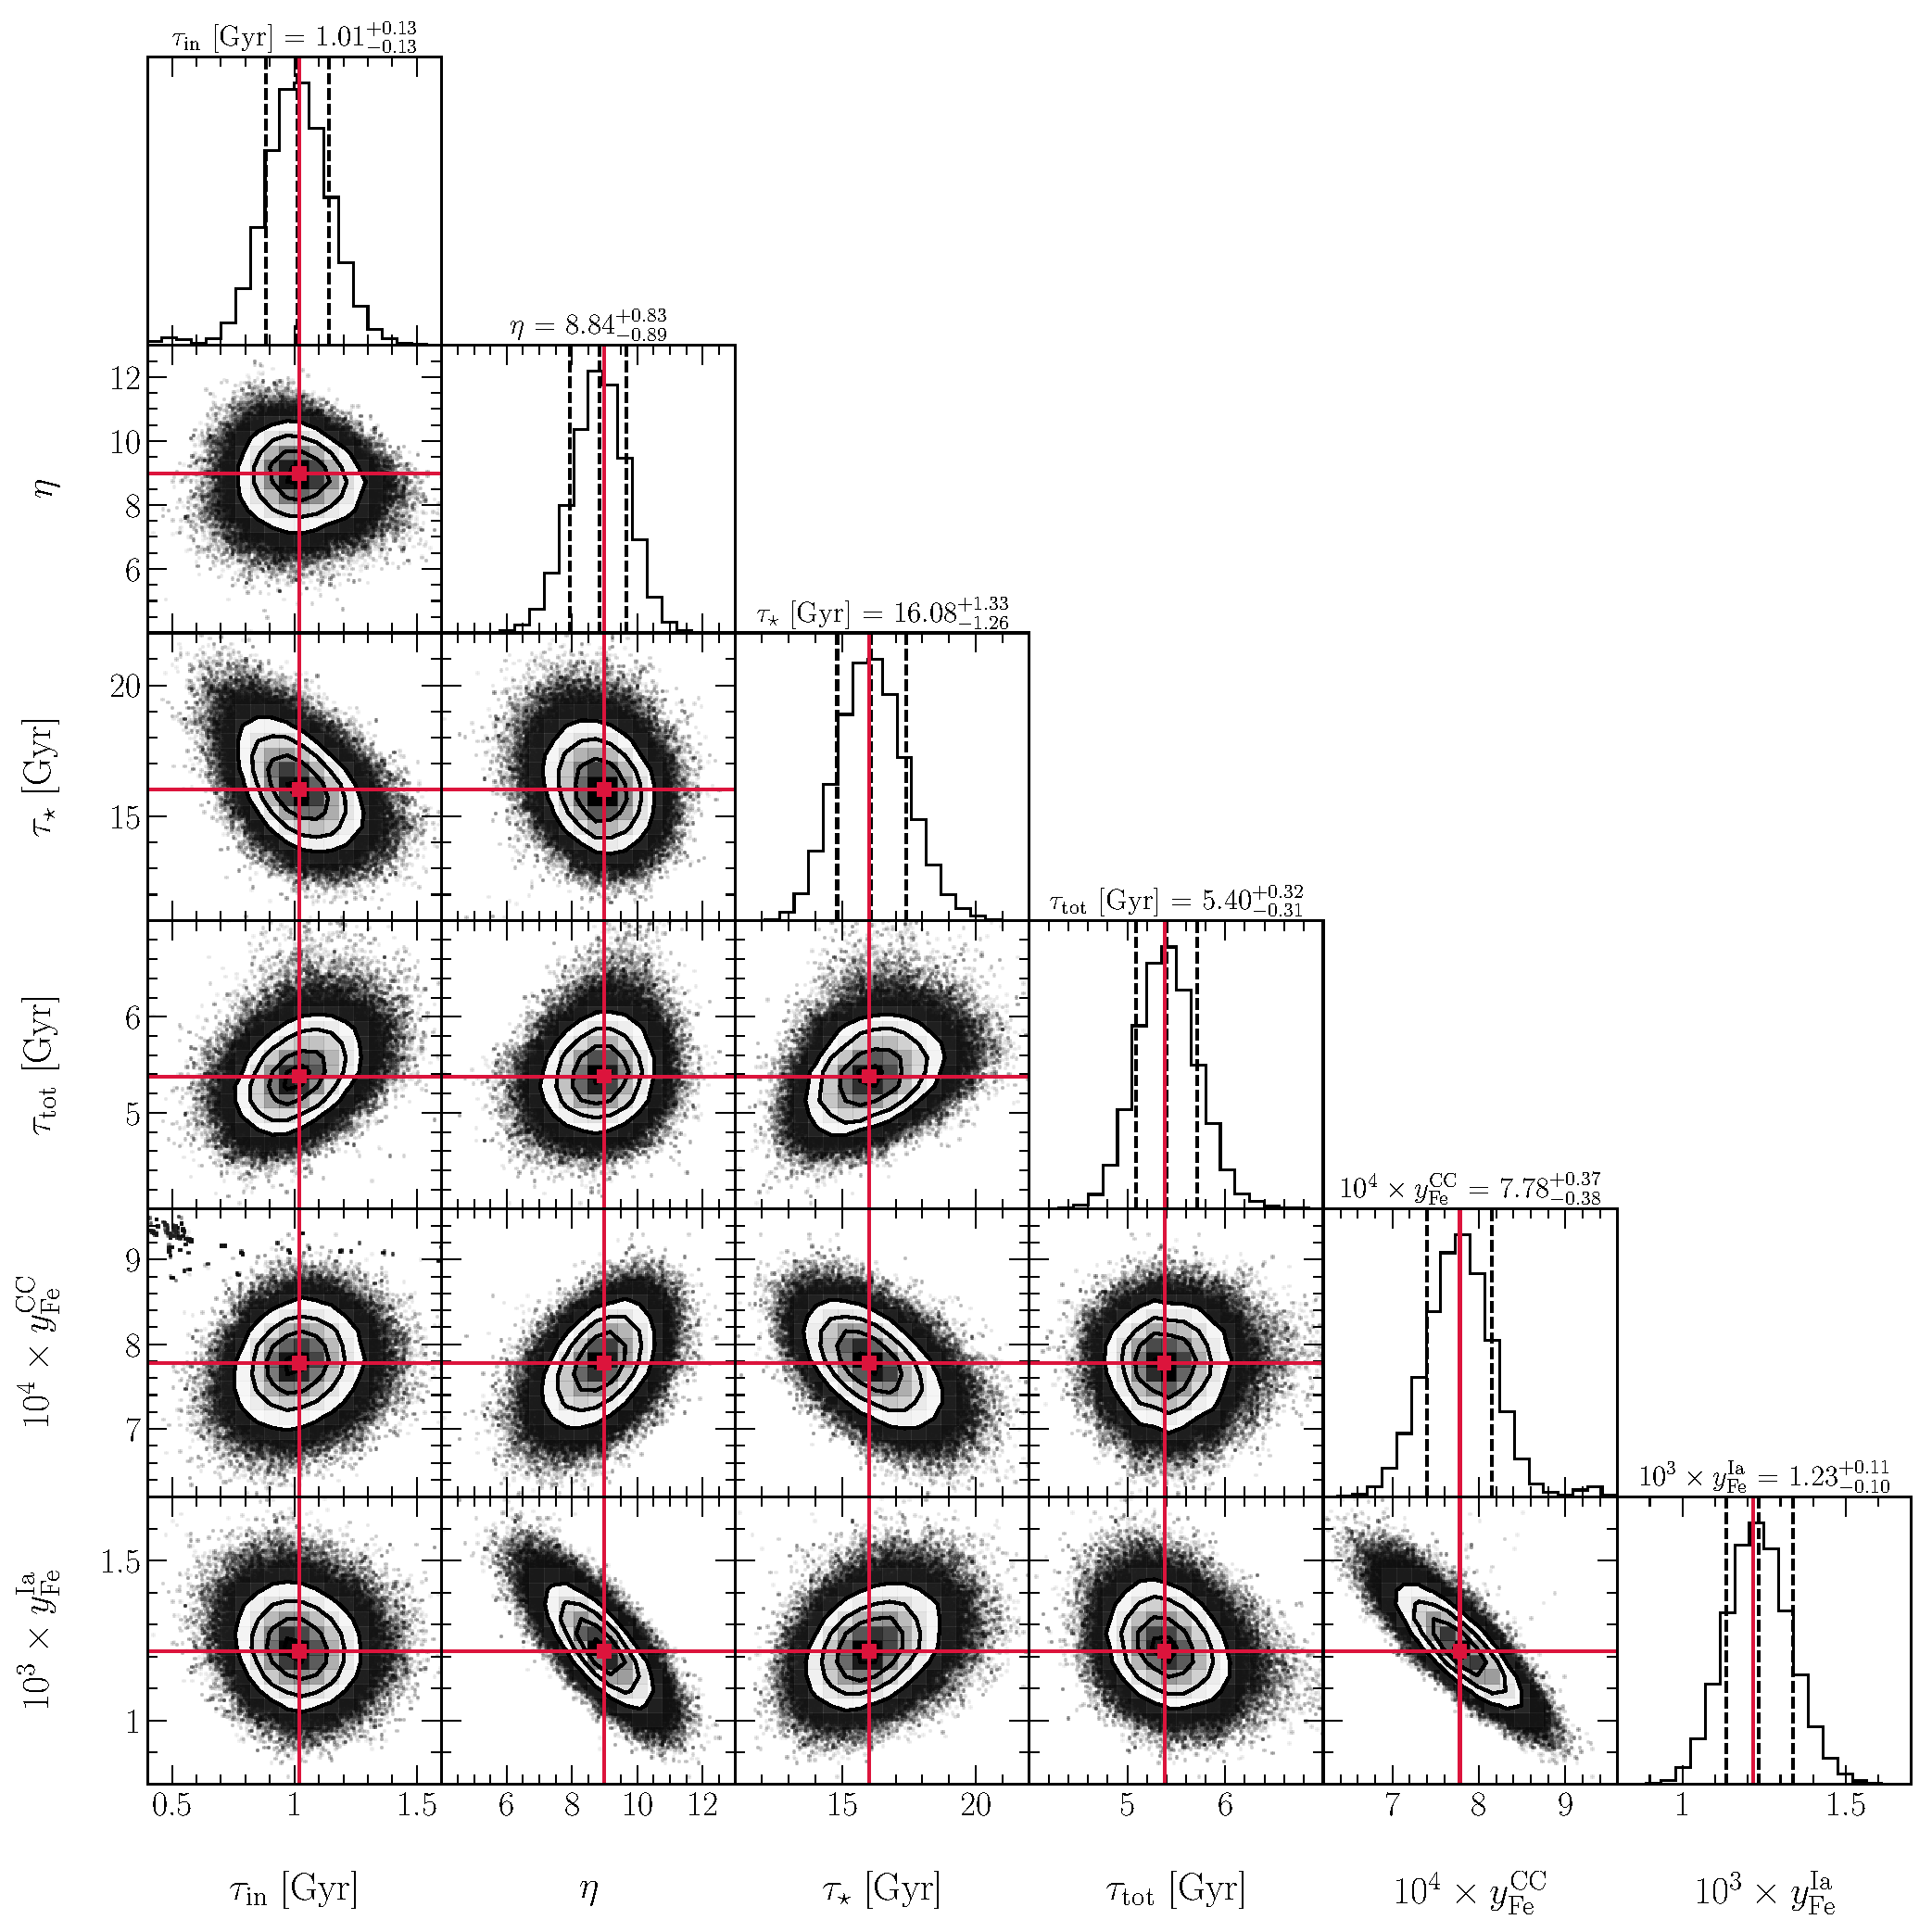
\includegraphics[scale = 0.45]{gsechem_512k.pdf}
\caption{
Posterior distributions for an exponential infall history applied to our GSE
sample.
The parametrization is the same as the input model to our mock samples (see
discussion in~\S~\ref{dga:sec:mocks:fiducial}).
Panels below the diagonal show 2-dimensional cross-sections of the likelihood
function while panels along the diagonal show the marginalized distributions
along with the best-fit values and confidence intervals.
Red ``cross-hairs'' mark the element of the Markov chain with the maximum
statistical likelihood.
The points in the upper left corner of the~$\yfecc - \tau_\text{in}$ plane
are a part of an extended tail of the likelihood distribution which does
not appear in other panels when zoomed in on the peak.
}
\label{dga:fig:gse_corner}
\end{figure*}

% fig 7
\begin{figure}
\centering
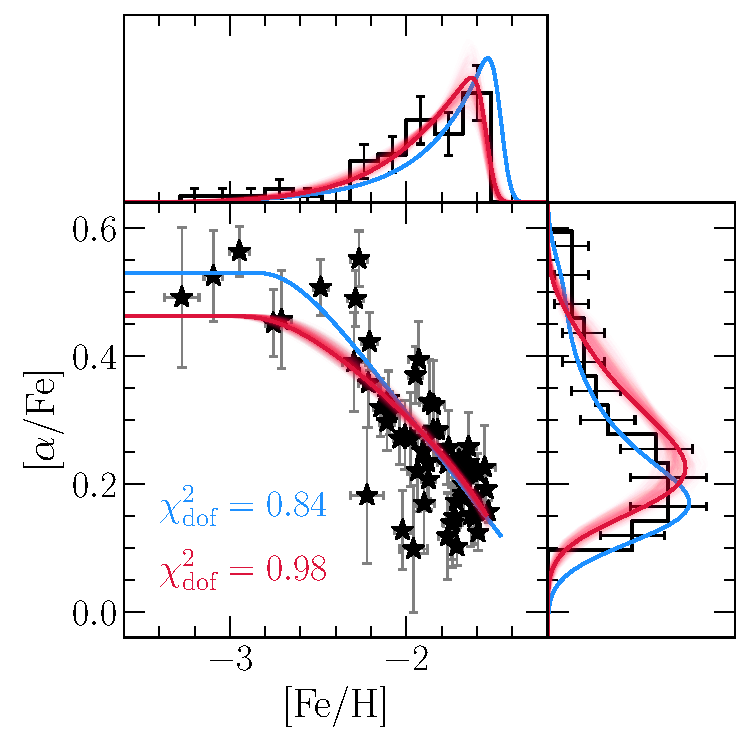
\includegraphics[scale = 0.65]{wukong_bestfit.pdf}
\caption{
Our Wukong/LMS-1 sample in the~\afe-\feh~plane and the associated marginalized
distributions.
Error bars indicate uncertainties on individual abundances in the central panel
and a~$\sigma = \sqrt{N}$ uncertainty from sampling noise in the top and right
panels.
Red lines denote our best-fit chemical evolution model (see discussion
in~\S~\ref{dga:sec:h3:wukong}), with 200 additional sets of parameter choices
subsampled from our Markov chain to give a sense of the fit precision.
Blue lines denote an alternate fit in which we allow the Fe yields to vary as
free parameters.
}
\label{dga:fig:wukong}
\end{figure}

% fig 8
\begin{figure*}
\centering
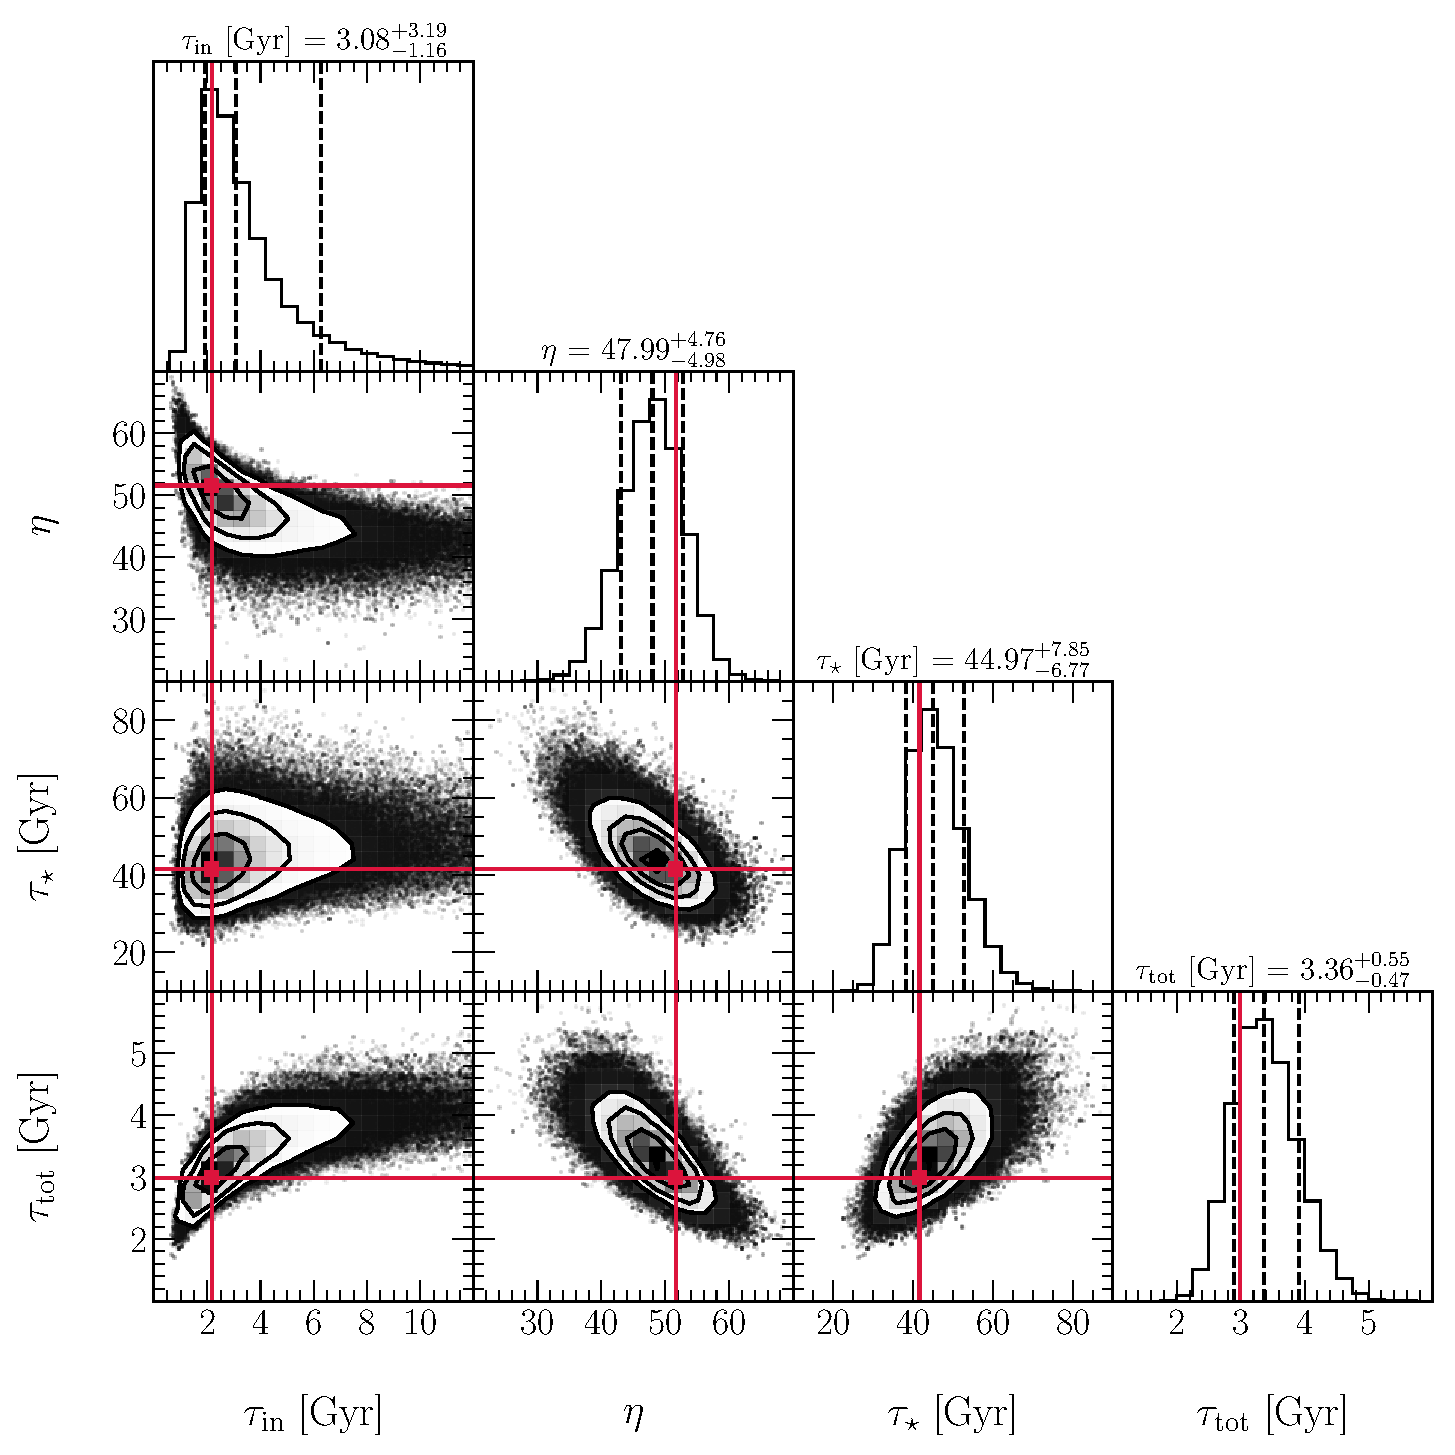
\includegraphics[scale = 0.6]{wukong_512k.pdf}
\caption{
Posterior distributions for an exponential infall history applied to our
Wukong/LMS-1 sample.
The parametrization is the same as the input model to our mock samples (see
discussion in~\S~\ref{dga:sec:mocks:fiducial}) but with the Fe yields held fixed
at the values determined by the fit to our GSE sample
($\yfecc = \scinote{7.78}{-4}$ and~$\yfeia = \scinote{1.23}{-3}$).
Panels below the diagonal show 2-dimensional cross-sections of the likelihood
function while panels along the diagonal show the marginalized distributions
along with the best-fit values and confidence intervals.
Red ``cross-hairs'' mark the element of the Markov chain with the maximum
statistical likelihood.
}
\label{dga:fig:wukong_corner}
\end{figure*}

We select our GSE sample based on the criteria in~\citet{Conroy2022}, which
yields a sample of 189 stars with spectroscopic signal-to-noise
SNR~$> 15$ and~\gaia~RUWE~$< 1.5$.
95 of them are main sequence turnoff and subgiant stars with surface gravities
of~$3.8 < \log g < 4.2$ with reliable age measurements.
Abundance uncertainties range from~$\sim$0.02 to 0.12 dex in
both~\feh~and~\afe~with median values near~$\sim$0.05.
Every age measurement has a statistical uncertainty
$\sigma_{\log_{10}(\text{age})} \leq 0.05$, corresponding to a measurement
precision of~$\lesssim$12\%.
However, due to the difficulty associated with measuring stellar ages both
accurately and precisely~\citep[e.g.,][]{Soderblom2010, Chaplin2013, Angus2019},
we adopt~$0.05$ as the age uncertainty for the entire sample to account for any
systematic errors that may be present.
\par
We illustrate our sample in Fig.~\ref{dga:fig:gse} along with our best-fit GCE
models (see discussion below).
We note the presence of two outliers at ages of~$\sim$5 and~$\sim$6 Gyr, marked
by X's in the right panel of Fig.~\ref{dga:fig:gse}.
With abundances typical of the rest of the GSE population but anomalously young
ages, these stars are likely blue stragglers, which are thought to be made
hotter and more luminous by accretion from a binary companion and biasing their
age measurements to low values~\citep[e.g.,][]{Bond1971, Stryker1993}.
It is also possible that these stars are high-eccentricity contaminants kicked
out of the disk by Sagittarius~\citep[e.g.,][]{Donlon2020}.
The smooth decline of~\afe~with~\feh~and the unimodal nature of the
distributions in~\feh,~\afe~and age indicate that the GSE did not experience
any significant starburst events.
If it had, we would expect to see a multi-peaked age distribution
as well as an increase in~\afe~at a distinct~\feh~due to the perturbed ratio of
CCSN to SN Ia rates~\citep{Johnson2020}.
We therefore fit the GSE with an exponential infall history (the same as our
mock samples explored in~\S~\ref{dga:sec:mocks}), omitting the two~$\sim$5
and~$\sim$6 Gyr old stars from the procedure and retaining the assumption that
star formation commenced 13.2 Gyr ago.
Because H3 selects targets based only on a magnitude range and a maximum
parallax, the selection function in chemical space should be nearly uniform
(i.e.,~$\script{S}(\script{M}_j | \{\theta\}) \approx 1$ for all points
$\script{M}_j$ along the evolutionary track.
We therefore take weights that are proportional to the SFR alone (see
equations~\ref{dga:eq:likelihood} and~\ref{dga:eq:weights} and discussion
in~\S~\ref{dga:sec:fitting}).
\par
We report our best-fit evolutionary parameters in Table~\ref{dga:tab:results}
with Fig.~\ref{dga:fig:gse_corner} illustrating the posterior distributions.
These values suggest strong outflows ($\eta \approx 9$) and inefficient star
formation ($\tau_\star \approx 16$ Gyr).
Invoking the equilibrium arguments of~\citet{Weinberg2017b}, strong outflows and
slow star formation are consistent with the metal-poor mode of the MDF and the
``knee'' in the evolutionary track occurring at low~\feh, respectively.
These results are expected for a dwarf galaxy where the gravity well is
intrinsically shallow and the stellar-to-halo mass ratios are known empirically
to be smaller than their higher mass counterparts~\citep{Hudson2015}.
The alpha-enhanced mode of the MDF reflects the short duration of star
formation, stopping before SN Ia enrichment could produce enough Fe to reach
solar~\afe.
The associated truncation of the age distribution (shown in the bottom left
panel of Fig.~\ref{dga:fig:gse}) likely reflects the quenching of star
formation in the GSE progenitor as a consequence of ram pressure stripping by
the hot halo of the Milky Way after its first infal~$\sim$10 Gyr ago
\citep{Bonaca2020}.
The inferred Fe yields suggest that massive stars account for
$\yfecc / (\yfecc + \yfeia) \approx 40$\% of the Fe in the universe.
These values may however be influenced by the H3 pipeline~\textsc{MINESweeper}
\citep{Cargile2020}, which includes a prior enforcing~$\afe \leq +0.6$ -- if
the~\afe~plateau occurs near this value in nature, this prior could bias the
most alpha-rich stars in our sample to slightly lower~\afe~ratios.
\par
Red lines in Fig.~\ref{dga:fig:gse} illustrate our best-fit model compared to the
data
Visually, this model is a reasonable description of the data, though in detail
it predicts a slightly broader~\feh~distribution and a slightly more peaked age
distribution.
We assess the quality of the fit with equation~\refp{dga:eq:chisquared_dof} and
find~$\chi_\text{dof}^2 = 1.34$, suggesting that this fit is indeed accurate
but that there may be some marginal room for improvement.
The substantial scatter in the age-metallicity relation (lower right panel)
arises due to the age uncertainties -- to clarify this point, we subsample 95
stars (the same number in our sample with age measurements) from our best-fit
SFH and perturb their implied ages and abundances by the median observational
uncertainties.
These random draws (red points) occupy a very similar region of the age-\feh~and
age-\afe~planes.
We do however note an additional~$\sim$6 or 7 potential blue stragglers with
ages of~$\sim$$8 - 9$ Gyr,~$\feh \approx -1.2$ and~$\afe \approx +0.4$.
These stars are less obviously blue stragglers than the~$\sim$5 and~$\sim$6 Gyr
old ones and would not have stood out without this comparison.
These stars likely play a role in increasing the~$\chi_\text{dof}^2$ of our
fit, and removing them from our sample would also bring the observed age
distribution into better agreement with our best-fit model.
We however do not explore more detailed investigations of individual stars for
fits to carefully tailored populations here, and the fit we obtain is
statistically reasonble anyway.
\par
In~\S~\ref{dga:sec:mocks:variations}, we found that our model accurately recovered
the evolutionary timescales of the input model even in the absence of age
information due to their impact on the shape of the MDF.
To assess the feasibility of deducing these parameters from abundances alone,
we conduct an additional fit to our GSE sample omitting the age measurements.
We report the best-fit parameters in Table~\ref{dga:tab:results}.
This procedure results in accurate fits to the~\feh~and~\afe~distributions, and
the SN yields and mass-loading factor~$\eta$ are generally consistent with
and without ages.
The inferred timescales are biased toward higher values and are discrepant
by~$\sim$$2\sigma$, with the duration of star formation showing the largest
difference.
These results indicate that such an approach is theoretically possible, but in
practice age information in some form is essential to pinning down these
timescales.
In~\S~\ref{dga:sec:mocks}, we fit our mock samples with the exact underlying GCE
model and same numerical code which integrated the input model, placing the
same systematic effects in the data as the model.
It is also never guaranteed that the evolutionary history built into the model
is an accurate description of the galaxy.
% While the most powerful way to provide age information for a fit under this
% procedure is with star-by-star measurements, that is difficult for external
% galaxies with current instrumentation and could instead be achieved with, e.g.,
% a CMD-derived SFH included as a prior.

\subsection{Wukong/LMS-1}
\label{dga:sec:h3:wukong}

% fig 9
\begin{figure}
\centering
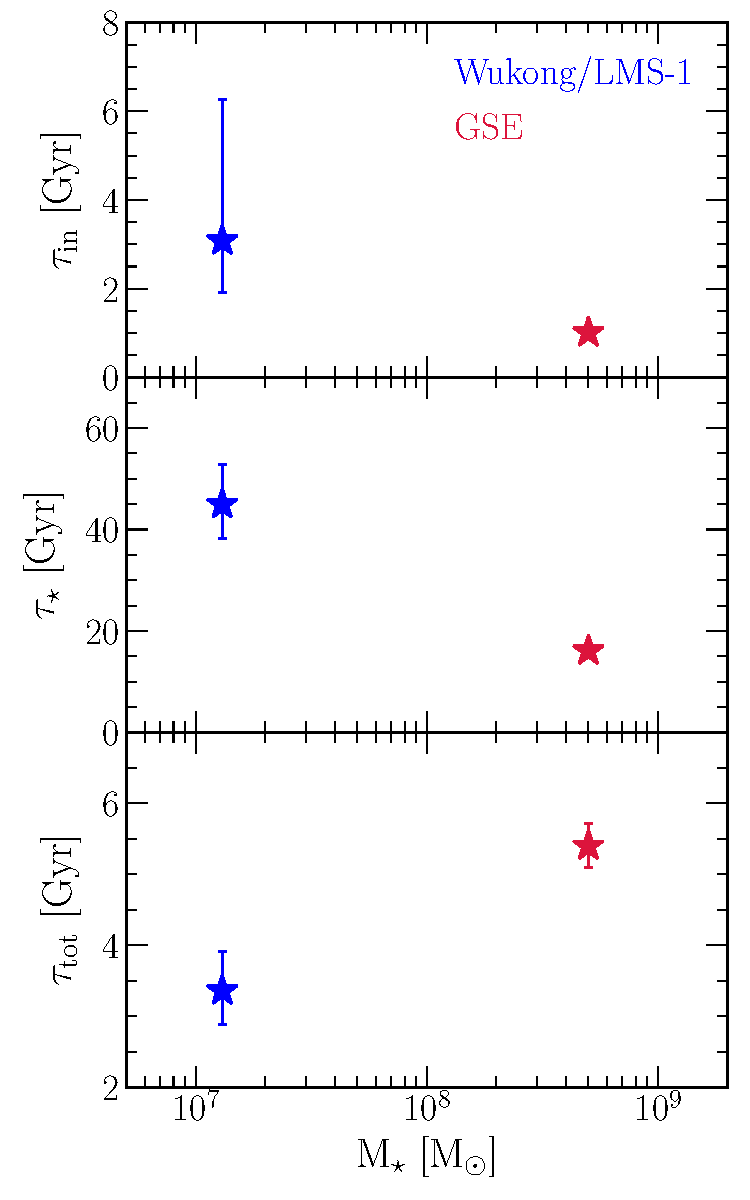
\includegraphics[scale = 0.63]{gse_wukong_timescales.pdf}
\caption{
Our best-fit evolutionary timescales for Wukong/LMS-1 (blue) and GSE (red) as a
function of their stellar mass (taken from~\citealt{Naidu2022}; values are
tabulated in Table~\ref{dga:tab:results}).
The uncertainties in the infall timescale~$\tau_\text{in}$ and the SFE
timescales~$\tau_\star$ for GSE are smaller than the point.
}
\label{dga:fig:gse_wukong_timescales}
\end{figure}

% fig 10
\begin{figure}
\centering
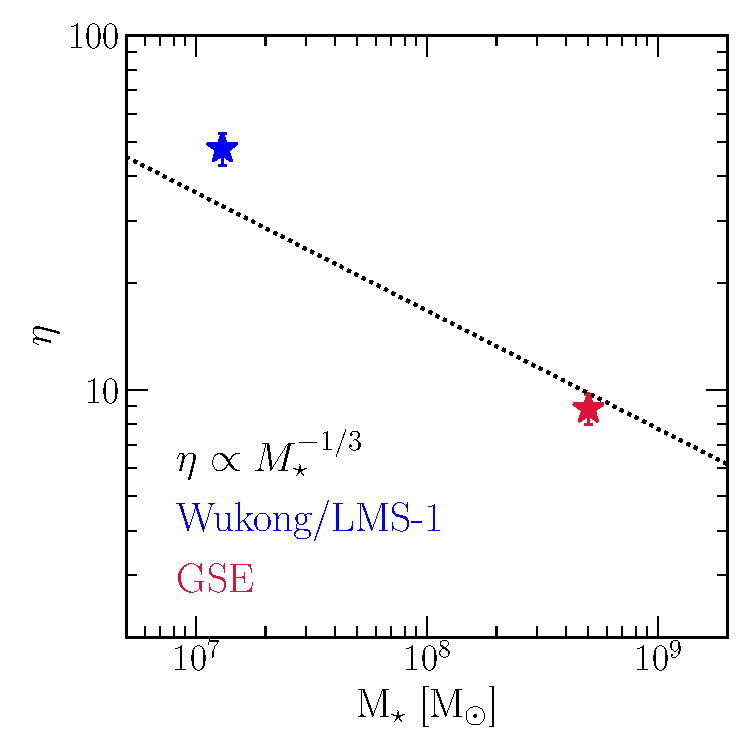
\includegraphics[scale = 0.6]{gse_wukong_eta.pdf}
\caption{
Our best-fit mass-loading factors~$\eta$ for Wukong/LMS-1 (blue) and GSE (red) as
a function of their stellar mass (taken from~\citealt{Naidu2022}; values are
tabulated in Table~\ref{dga:tab:results}).
The black dashed line denotes~$\eta \propto M_\star^{-1/3}$ as suggested by
\citet{Finlator2008} and~\citet{Peeples2011} with the normalization of
$\eta = 3.6$ at~$M_\star = 10^{10}~M_\odot$ taken from~\citet{Muratov2015}.
}
\label{dga:fig:gse_wukong_eta}
\end{figure}

We select Wukong/LMS-1 stars following the criteria in~\citet{Naidu2020}, with
the following additional cuts for high purity (inspired by the orbits of the
accomparnying globular clusters, NGC 5024 and NGC 5053, and~\citealt{Yuan2020}
and~\citealt{Malhan2021} who made selections based on the orbital plane):
\begin{itemize}

	\item[\textbf{1.}] $(J_z - J_r) / J_\text{tot}$ > 0.7, where~$J$ is action.

	\item[\textbf{2.}] $90^\circ < \theta < 120^\circ$, where~$\theta$ and
	$\phi$ are angles defining the angular momentum unit vector.

\end{itemize}
The~\citet{Naidu2020} selection features a hard cut at~$\feh < -1.45$ to avoid
GSE contamination, but visual inspection of the Wukong/LMS-1 sequence in
the~\afe-\feh~plane indicates that it drops off around~$\feh \approx -1.5$,
(see Fig.~\ref{dga:fig:wukong}) and high [$\alpha$/Fe] GSE stars appear at higher
metallicities.
Our sample consists of 57 stars with spectroscopic SNR~$> 10$
and~\gaia~RUWE~$< 1.5$, none of which have age information as they are all
distant halo stars.
Within this sample, 23 stars are at SNR~$> 20$ and the remaining 34 are at
$10 <$ SNR~$< 20$.
Abundance uncertainties range from~$\sim$0.02 to~$\sim$0.10 dex in
both~\afe~and~\feh~with median values near~$\sim$0.045.
\par
Fig.~\ref{dga:fig:wukong} illustrates this sample in chemical space along with our
best-fit GCE model (see discussion below).
Similar to the GSE, the lack of discontinuities in the age and abundance trends
indicates a smooth SFH devoid of any starburst events.
We therefore fit this sample with the same exponential infall history as the
input model to our mock samples, which we also applied to our GSE data.
We retain the assumption that star formation began 13.2 Gyr ago and that the H3
selection function is uniform in chemical space (see discussion
in~\S~\ref{dga:sec:h3:gse}).
However, due to the smaller sample size and the lack of age information, we
initially hold our Fe yields fixed at~$\yfecc = \scinote{7.78}{-3}$ and
$\yfeia = \scinote{1.23}{-3}$ as suggested by the fit to our GSE sample.
It is reasonable to expect SN yields to be the same from galaxy-to-galaxy since
they are set by stellar as opposed to galactic physics, though we explore the
impact of relaxing this assumption below.
\par
Table~\ref{dga:tab:results} reports the inferred best-fit parameters and
Fig.~\ref{dga:fig:wukong_corner} illustrates the posterior distributions.
The degeneracies between parameters are noticeably more asymmetric than in our
GSE sample, a result of the lack of age information (we found similar effects
in our tests against mock data in~\S~\ref{dga:sec:mocks}, though we did not discuss
it there).
The e-folding timescale of the accretion rate in particular has a highly skewed
likelihood distribution ($\tau_\text{in} = 3.08^{+3.19}_{-1.16}$ Gyr).
We have also had reasonable success describing Wukong/LMS-1 with a constant
star formation history.
Consequently, the likelihood function has a tail that extends
to~$\tau_\text{in} \rightarrow \infty$.
The exponential infall history is indeed a statistically better fit, so
throughout this section we include a prior that
enforces~$\tau_\text{in} \leq 50$ Gyr to focus on this portion of parameter
space.
This tail is significantly more extended if the Fe yields are allowed to vary
as a free parameter (see Table~\ref{dga:tab:results} and discussion below).
\par
An exponential infall history yields a statistically good fit
($\chi_\text{dof}^2 = 0.98$; equation~\ref{dga:eq:chisquared_dof}) for Wukong/LMS-1,
though visually it appears that the SN yields implied by our GSE data
underestimate the height of the [$\alpha$/Fe] plateau, which we indirectly
held fixed via the Fe yields.
Although we asserted above that it is reasonable expect SN yields to be the
same between Wukong/LMS-1 and GSE, variations in the plateau height could
indicate either metallicity-dependent yields or variations in the IMF.
To investigate this hypothesis, we conduct an additional fit where we allow
the Fe yields to vary as free parameters, reporting the results in
Table~\ref{dga:tab:results} and illustrating the deduced model for comparison in
Fig.~\ref{dga:fig:wukong}.
A higher plateau indeed provides an even better fit
($\chi_\text{dof}^2 = 0.84$), but with~$\chi_\text{dof}^2$ less than 1, this
could be an overparametrization of the data.
This possibility is not necessarily to a worrisome extent though; we cannot
rule out either model.
The best-fit SFE timescales between the two fits are in excellent agreement,
indicating that~$\tau_\star$ does not significantly impact the height of the
plateau (to first-order, it determines the position of the knee in the
track;~\citealp{Weinberg2017b}).

\subsection{Comparison}
\label{dga:sec:h3:comparison}

Fig.~\ref{dga:fig:gse_wukong_timescales} compares the best-fit evolutionary
timescales between GSE and Wukong/LMS-1 as a function of their stellar mass (we
adopt the stellar masses inferred by~\citealt{Naidu2021, Naidu2022}; our GCE
models as we have parametrized them do not offer any constraints on this
quantity).
Due to the yield-outflow degeneracy (see Appendix~\ref{dga:sec:degeneracy}), only
relative values of~$\tau_\star$ carry meaning, while the absolute values of
$\tau_\text{in}$ and~$\tau_\text{tot}$ do.
Qualitatively consistent with semi-analytic models of galaxy formation
\citep[e.g.,][]{Baugh2006, Somerville2015a, Behroozi2019} and results from
hydrodynamical simulations~\citep[e.g.,][]{GarrisonKimmel2019}, the less
massive of the two galaxies experienced the more extended accretion history.
Star formation in Wukong/LMS-1, however, was less efficient and did not last as
long as in GSE -- sensible results given the empirical correlation between
stellar-to-halo mass ratioes and stellar mass~\citep{Hudson2015}.
To the extent that our one-zone model framework is accurate, we have
constrained the duration of star formation in Wukong/LMS-1 and GSE to 15.2\%
and 5.8\%, respectively.
However, our Wukong/LMS-1 sample has no age measurements, and we have not
derived an SFH from its CMD here.
The failure of our fit to GSE omitting all ages (see Table~\ref{dga:tab:results})
suggests that these best-fit parameters may be biased to high values.
\par
As expected given Wukong/LMS-1's shallower gravity well, it experienced
stronger mass-loading than GSE.
Fig.~\ref{dga:fig:gse_wukong_eta} shows the inferred mass-loading factors in
comparison to the scaling of~$\eta \propto M_\star^{-1/3}$ as suggested by
\citet{Finlator2008} and~\citet{Peeples2011} modelling the impact of galactic
winds on the mass-metallicity realtion for galaxies.
We take the normalization of~$\eta = 3.6$ at~$M_\star = 10^{10}~M_\odot$ from
\citet{Muratov2015} who find a similar scaling in the FIRE simulations
($\eta \propto M_\star^{-0.35}$;~\citealp{Hopkins2014}).
There is excellent agreement between this predicted scaling and our one-zone
model fits -- rather remarkably so given that we have made no deliberate
choices for either the normalization or the slope to agree.
\par
In Fig.~\ref{dga:fig:comparison}, we compare our best-fit models for GSE and
Wukong/LMS-1.
The intrinsic age distribution of GSE is predicted with considerably higher
precision than for Wukong/LMS-1, a consequence of the lack of age information
in our Wukong/LMS-1 sample.
The uncertainties in the Wukong/LMS-1 age distribution are noticeably
asymmetric due to the skewed posterior distribution of the infall timescale
($\tau_\text{in} = 3.08^{+3.19}_{-1.16}$ Gyr).
If our assumption that star formation began~$T \approx 13.2$ Gyr ago (see
discussion in~\S~\ref{dga:sec:mocks:fiducial}) is accurate for Wukong/LMS-1, then
it experienced quenching~$\sim$2 Gyr earlier than the GSE ($\sim$9.8 versus
$\sim$7.8 Gyr ago).
However, because we do not have age information for Wukong/LMS-1, this
distribution could shift uniformly to lower values with affecting the quality
of the fit.
Constraints on the centroid of the distribution could be derived by
analysing the CMD as in, e.g.,~\citet{Dolphin2002} and~\citet{Weisz2014b}, but
we do not pursue this method in the present paper as it involves an entirely
separate mathematical framework.
\par
Also as a consequence of the lack of age information, our fits constrain the
intrinsic age-\feh~and age-\afe~relations to somewhat higher precision for GSE
than Wukong/LMS-1.
While the age-\feh~relations are significantly offset from one another, the
predicted age-\afe~relations are remarkably consistent with one another.
A portion of this agreement can likely be traced back to our fixing the Fe
yields in our fit to Wukong/LMS-1 to the values inferred in our fit to GSE.
Nonetheless, it is reasonable to assume that the SN yields are the same between
the two galaxies because this should be set by stellar physics, sufficiently
decoupled from the galactic environment.
The evolution of~\afe~with time is in principle impacted by the various
evolutionary timescales at play, so their consistency with one another is still
noteworthy.

